\chapter{Modular Development of Embedded System}

Before an embedded CMS can be developed, it is necessary to test the individual elements in controlled conditions.
This will lead to confidence in the implementation of more sophisticated techniques which are necessary for CM.
\par

The processor used in this project is the MSP432P401R, mounted on a development board.
It was chosen for its: ease of development; low cost; Precision ADC; hardware pin configurations; EnergyTrace technology \cite{MSP432_Launchpad}.

\section{Online Processing}

On-board processing of data is a key component of the embedded CMS.
In addition to correctly transforming the signal from the time to frequency domain, statistics of the frequency spectrum must be correctly extracted.
As discussed previously, the parameters of maximum, RMS, and std have been chosen.
To assess the implementation of the processing, data generated and processed in Matlab is sent to the board to compare the output of processing.
It is expected that there will be some small differences in the results from the board and from Matlab.
The computation in Matlab will use double-precision floating-point format, whereas, to conserve memory use, 16 bit integers are used on-board.
The integers represent fixed point numbers and can suffer from both truncation and overflow errors \cite{Qmath}.
Fixed-point FFT has been studied and shown to have good accuracy, with mitigation strategies available to improve the signal-to-noise ration if necessary \cite{Fixed_point_FFT}\cite{Fixed_point_FFT_accuracy}.
To allow direct comparisons of the processing, the time domain input will be stored as integer values for both the board and Matlab.
\par

The on-board implementation uses the KissFFT library which is publically available under a BSD license \cite{KissFFT}.
KissFFT uses an out-of-place, time decimation, mixed-radix FFT and provides optimisation for even length real signals.
It also provides improved capability over freeware provided by the CMSIS-DSP library which limited the length of the time signal to 1024 \cite{CMSIS_DSP}.
There is no such limit with KissFFT which allows full use of the available on-board memory.
The MSP432 has 64 KB of SRAM \cite{MSP432_Launchpad}, so the theoretical limit for the sample size is $~(64000 / 3 / 2) = 10667$ - 1 array of real numbers as input, 1 array of real numbers and imaginary numbers each as output, and 2 bytes each for 16 bit integers.
However, the practical limit was found to be closer to 6000, due to how SRAM data and memory is allocated on the MSP432.
A sample size of 4096 is used as it provides an exact fraction of the available sampling rates and therefore a sensible resolution in the frequency domain.


\subsubsection{Results}

The results of processing a noisy time signal with multiple components are shown in Table \ref{tab:processing} and Fig \ref{fig:processing} and provide evidence that the on-board processing is accurate.
Limitations of this test are that the time signal is relatively simple, with five frequency components and noise.
At low levels of magnitude the on-board processing does not agree exactly with the Matlab output, however this does not interfere significantly with statistic extraction.

\begin{figure}
    \centering
    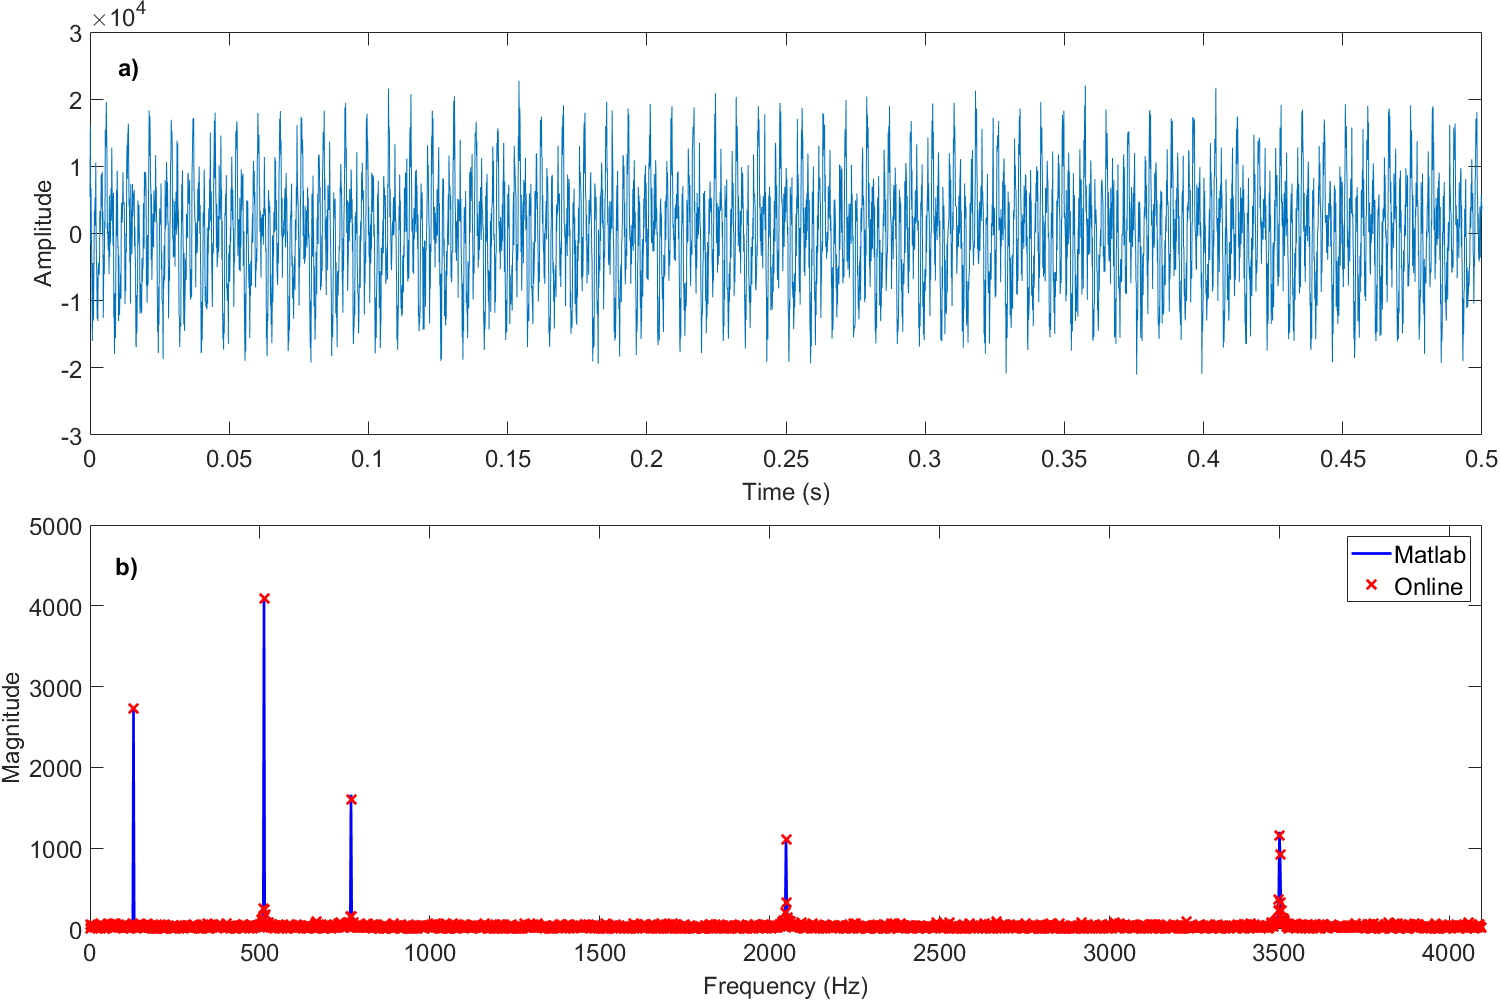
\includegraphics[width=\linewidth]{Processing.png}
    \caption{Processing of frequency spectrum in Matlab and on-board embedded system - a) Time signal, b) Frequency Spectrum}
    \label{fig:processing}
\end{figure}

\begin{table}
	\begin{center}
		\begin{tabular}{llll}%Changed c to S
			\toprule
			\textbf{Statistic}  & \textbf{Matlab} & \textbf{On-board}\\
			\midrule
			Maximum & 4078.20 & 4126 \\
			RMS & 127.27 & 128 \\
			Standard Deviation & 122.05 & 123  \\
			\bottomrule
		\end{tabular}
		\caption{Statistics of frequency spectrum calculated in Matlab and on-board from signal shown in Fig \ref{fig:processing}}
		\label{tab:processing}%Can be referenced by rest of document
	\end{center}
\end{table}

\section{ADC}

Having demonstrated the capability of the on-board processing, the next step is to combine it with analog inputs at specific sampling frequencies and compare the output with a model signal generated in Matlab.
Many accelerometers and current sensors provide analog outputs only so verifying the accuracy of this module is key to obtaining reliable data from more complex measurements with peripherals.
\par

\begin{figure}
    \centering
    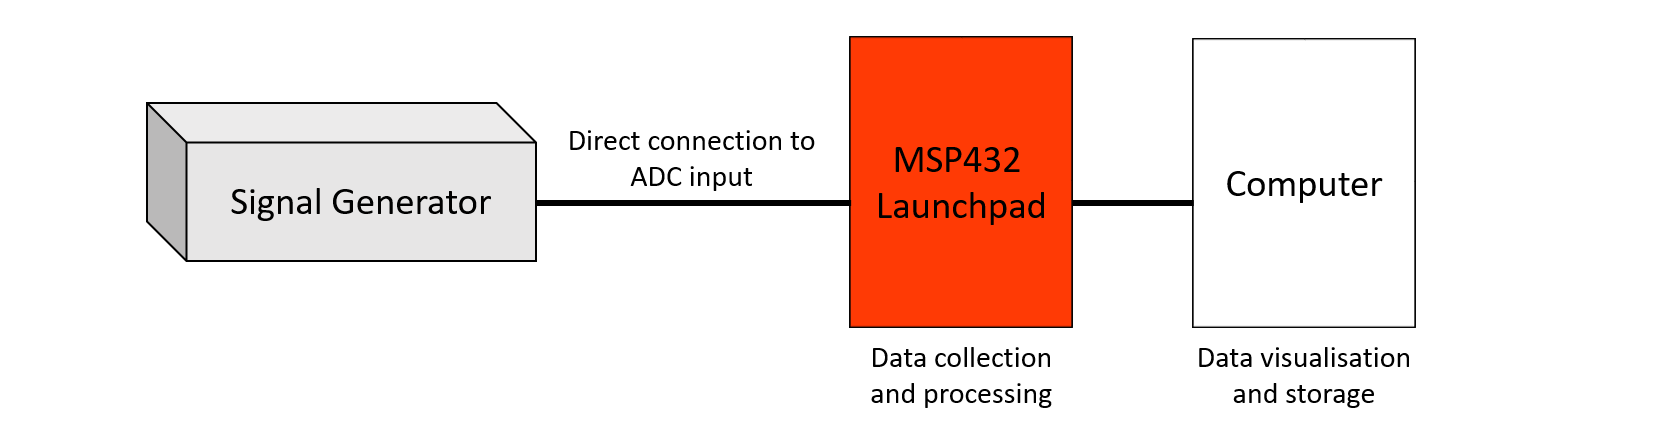
\includegraphics[width=\linewidth]{TestSetup2.PNG}
    \caption{Test setup for ADC measurements}
    \label{fig:ADCtest}
\end{figure}

MSP432 has an Analogue-to-Digital Converter (ADC) which measures with 14 bits (0 - 16833) and can be triggered from a number of internal clocks \cite{MSP432_Datasheet}.
While the advertised maximum sampling rate is 1 Million Samples Per Second (MSPS) it was found through experimentation that the most accurate timing source is the internal low-frequency oscillator in its 32.768 kHz mode.
Due to the way the timing trigger works for the ADC, the maximum sampling frequency with this oscillator is 16384 Hz, giving a Nyquist frequency of 8192 Hz.
While this is less than the 10 kHz range recommended for full condition monitoring, it will still be effective for diagnosing a wide range of faults and performing other condition monitoring services \cite{ISO13373-1}\cite{CBM_lr}.
The ADC measures from 0 V to $V_{cc}$, which is 3.3 V for the MSP432 \cite{MSP432_Datasheet}.
\par
To test the ADC, a Rigol DG1062Z signal generator provided sinusoid signals directly to the analog input pins of the MSP432 (Fig \ref{fig:ADCtest}).
Frequencies were chosen to be offset by 53 Hz to avoid harmonics of the supply frequency \cite{MEMS_testing}.
The amplitude of the signal is 1 V peak-to-peak and offset by 1.5 V to prevent breaching the limits of the ADC.
The DC component produced by the offset was removed during pre-processing of the time signal on-board - subtracting the mean of the time signal from each value.
Model signals were generated in Matlab for comparison, with the same sampling frequency and scaling the amplitude by $(V_{pp} / V_{cc})* bits_{adc}$.



\subsubsection{Results}

The results of the frequencies tested are shown overlaid on a single graph, against the peak value calculated by the model (Fig \ref{fig:ADC_experiment}).
There is good agreement with the model signals.
In particular, the frequency is identified well and the amplitude is similar for most values.
It can be seen that there are no peaks between the measured frequencies, indicating that both the measurement and FFT functions are working as expected.
It was found that at high frequencies, more than 6 kHz, the amplitude of the signal measured was not constant with time.
This suggests there are small inaccuracies with the ADC at higher frequencies.
Overall, this experiment demonstrates good functionality of the embedded system to measure and evaluate signals across a range of frequencies relevant to condition monitoring.



\begin{figure}
    \centering
    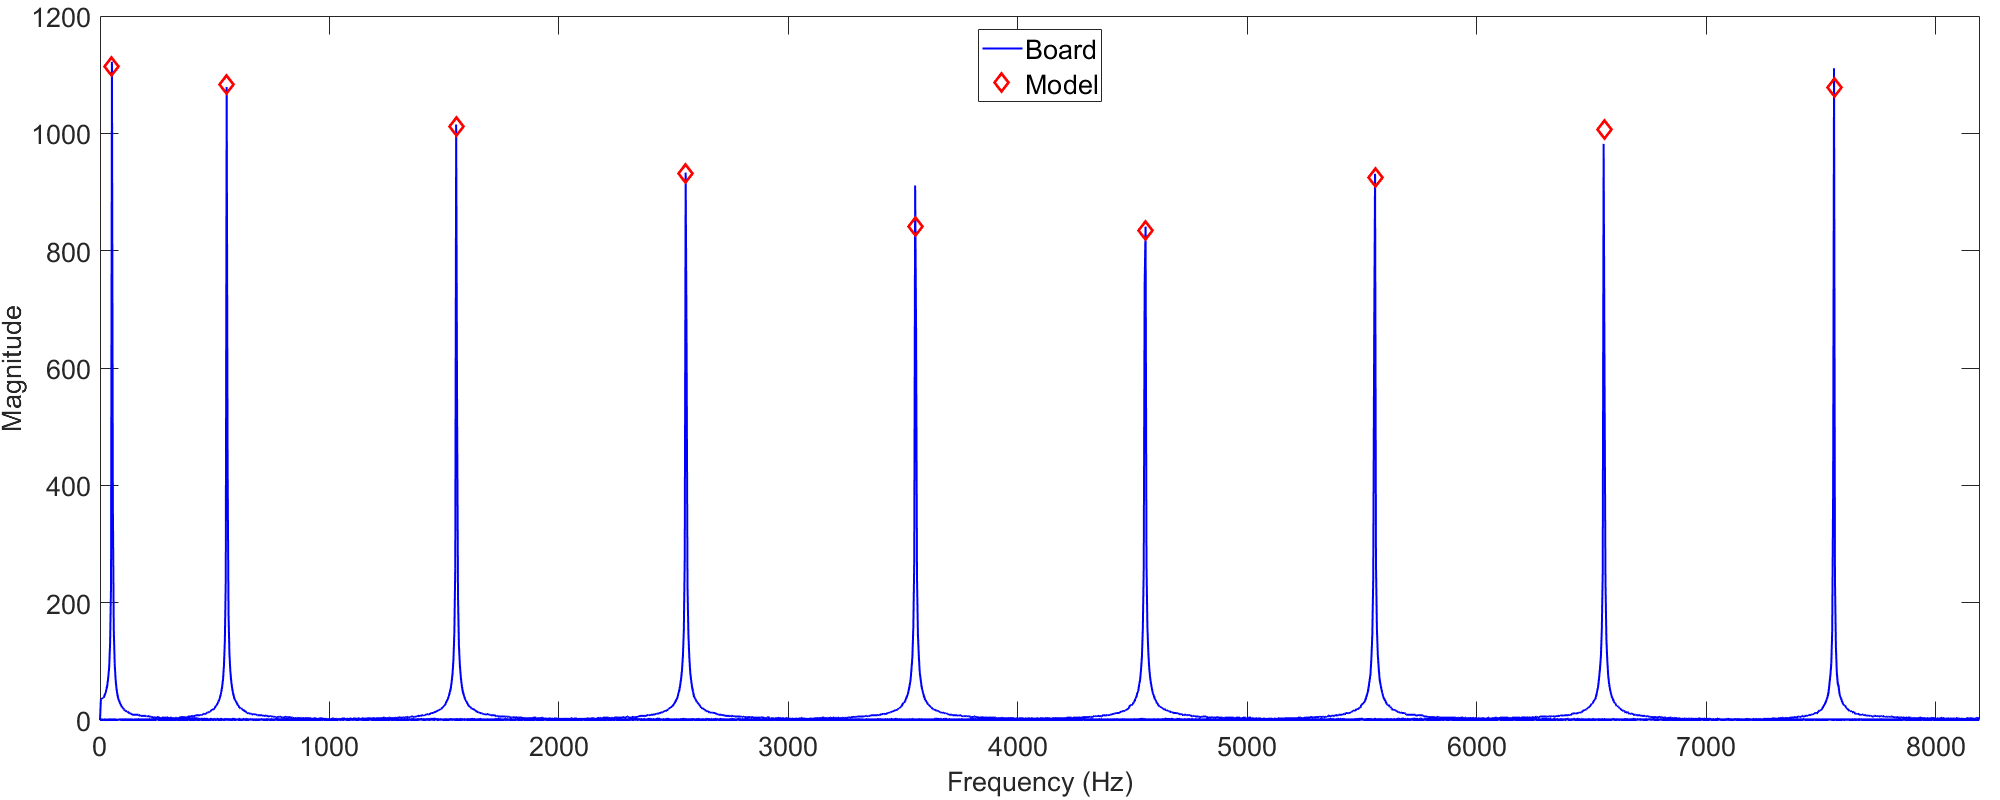
\includegraphics[width=\linewidth]{ADC_experiment.png}
    \caption{Processing of frequency spectrum in Matlab and on-board embedded system - a) Time signal, b) Frequency Spectrum}
    \label{fig:ADC_experiment}
\end{figure}


\section{Accelerometers}

Three accelerometers were identified which are suitable for the embedded system and which will provide useful information about the state of the accelerometer market with respect to the needs of CBM systems.
Microelectromechanical system (MEMS) accelerometers are often cheaper and smaller than their piezoelectric counterparts, and have been shown to work well measuring amplitude and frequency of vibration \cite{MEMS_testing}.
The accelerometers chosen have significantly different bandwidths, the frequency at which response is -3 dB from the true value.
They also have a range of sensitivities.
All three provide analogue output and operate at 3.3 V.
The properties are outlined in full in Table \ref{tab:MEMS}.
\par

To test the devices, the accelerometers were vibrated at a known frequency and power and their responses compared, similar to methods described in \cite{MEMS_testing}\cite{MEMS_testing2}.
The setup is shown in Fig \ref{fig:Acc_Test_Setup}.
A Rigol DG1062Z signal generator is connected to a Frederiksen 2185.00 Vibration Generator.
The vibration generator can vibrate at signals from 0.1 Hz to 5 kHz with amplitude of 7 mm at low frequencies and decreasing with frequency \cite{Frederiksen}.
Sinusoidal signals were generated to provide a clear signal.
%Accelerometers were fixed to the vibration generator using a specially manufactured banana plug fixing (Fig \ref{fig:Banana}) to ensure  \cite{Smart_Bearings_1}.
A specially manufactured banana plug (Fig \ref{fig:Banana}) provided a strong mechanical fixing for the accelerometers to ensure accurate readings \cite{Smart_Bearings_1}.
As the accelerometers were mounted on evaluation boards, screw holes closest to the ICs were used to mitigate the effects of resonance of the boards themselves, although this effect could not be completely removed.
The sensor output is connected to the MSP432 analog input, which collects data and performs data processing on the signal.
The time data and frequency signal are then sent to the computer for data visualisation, storage and further processing.
\par

The main subject of interest in this experiment is how the accelerometers respond at different frequencies.
To avoid interference from the mains frequency, the frequencies chosen were offsets of 53 Hz \cite{MEMS_testing}.
A low frequency within the frequency range of all the accelerometers was tested, followed by multiples of 500 Hz.
The signal generator was set to a peak-to-peak voltage of 5 V which was found to produce vibrations of approximately $\pm 1 g$ RMS.
Beyond 2553 Hz, the acceleration increased significantly beyond the range of two sensors, so testing was limited to these frequencies.
\par

The accelerometer output was sampled at 16384 Hz, significantly higher than the highest frequency to be tested.
Each measurement period collected 4096 samples, giving a frequency resolution of 4 Hz.
Three samples were collected from each accelerometer at each frequency, and the RMS acceleration and maximum of the frequency spectrum was averaged across the samples.
Using RMS and averaging the frequency spectrum are both methods which will reduce the effect of noise in the measurements and allow the true performance of the sensors to be assessed \cite{CM_randall}.
ADC values were converted to standard units using the theoretical sensitivities listed in the datasheets of the accelerometers \cite{MMA7361}\cite{ADXL354}\cite{ADXL1002}.
It is expected that MEMS A will show attenuated response at high frequencies compared to MEMS B and C due to its lower frequency range.
Effects due to resonance may also be visible in the higher frequency tests of MEMS B \cite{ADXL354}.
Inaccuracies are expected for C as the acceleration is small compared to the range of the sensor and resolution will therefore be lower than A and B.
\par

The experiment was performed in the Hardware Lab in Zepler Building at University of Southampton.
Other experiments and work was being performed at the same time which could contribute noise to the results.
The temperature inside the lab is maintained at a constant temperature of 22\textdegree{}C, but variations in temperature could also add inaccuracy to the measurements.

\begin{savenotes}
\begin{table}
    \renewcommand{\arraystretch}{1.5}
	\begin{center}
		\begin{tabular}{llll}%Changed c to S
			\toprule
			  & \textbf{A} & \textbf{B} & \textbf{C}  \\
			\midrule
			\textbf{Sensitivity (mV/g} & 800 & 400 & 40 \\
			\textbf{Frequency Range (kHz)} & 0.400 & 1.500 & 11\\
			\textbf{Amplitude Limit (g)} & $\pm 1.5$ & $\pm 2$ & $\pm 50$\\
			\textbf{Resonant Frequency (kHz)} & 6.0 & 2.4 & 21\\
			\textbf{Shock Limit (g)} & 5000 & 5000 & 10000\\
			\textbf{Unit Price (£)\footnote{Unit price for single evaluation board at large UK electrical retailer}} & N/A\footnote{No longer on sale} & 38.15 & 73.76\\
			\bottomrule
		\end{tabular}
		\caption{Properties of MEMS accelerometers \cite{ADXL354}\cite{MMA7361}\cite{ADXL1002}}
		\label{tab:MEMS}%Can be referenced by rest of document
	\end{center}
\end{table}
\end{savenotes}

\begin{figure}
    \centering
    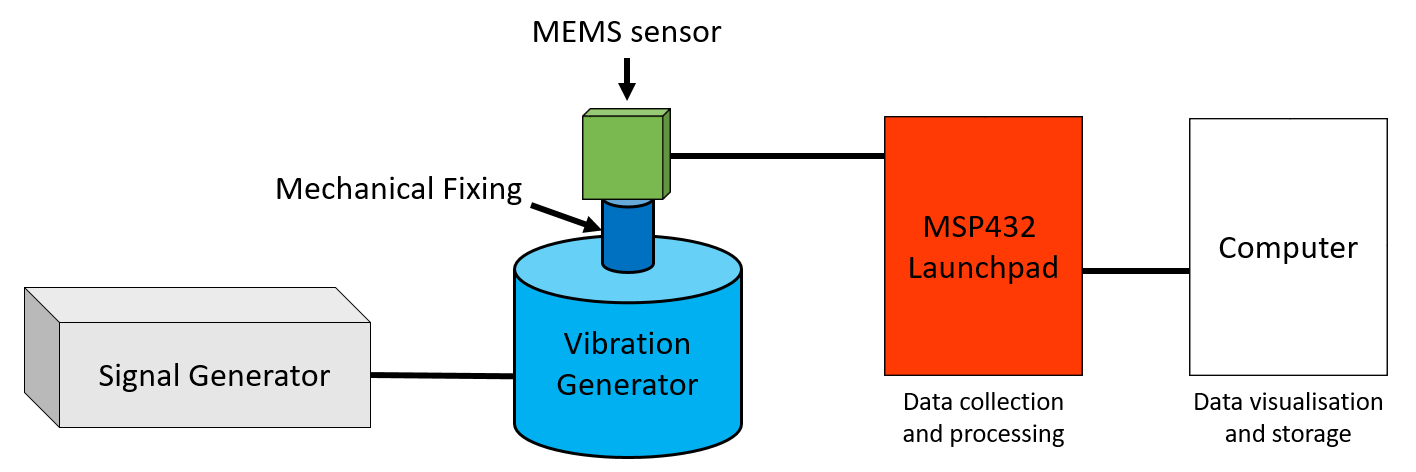
\includegraphics[width=\linewidth]{TestSetup1.png}
    \caption{Setup for testing MEMS accelerometers}
    \label{fig:Acc_Test_Setup}
\end{figure}

\begin{figure}
    \centering
    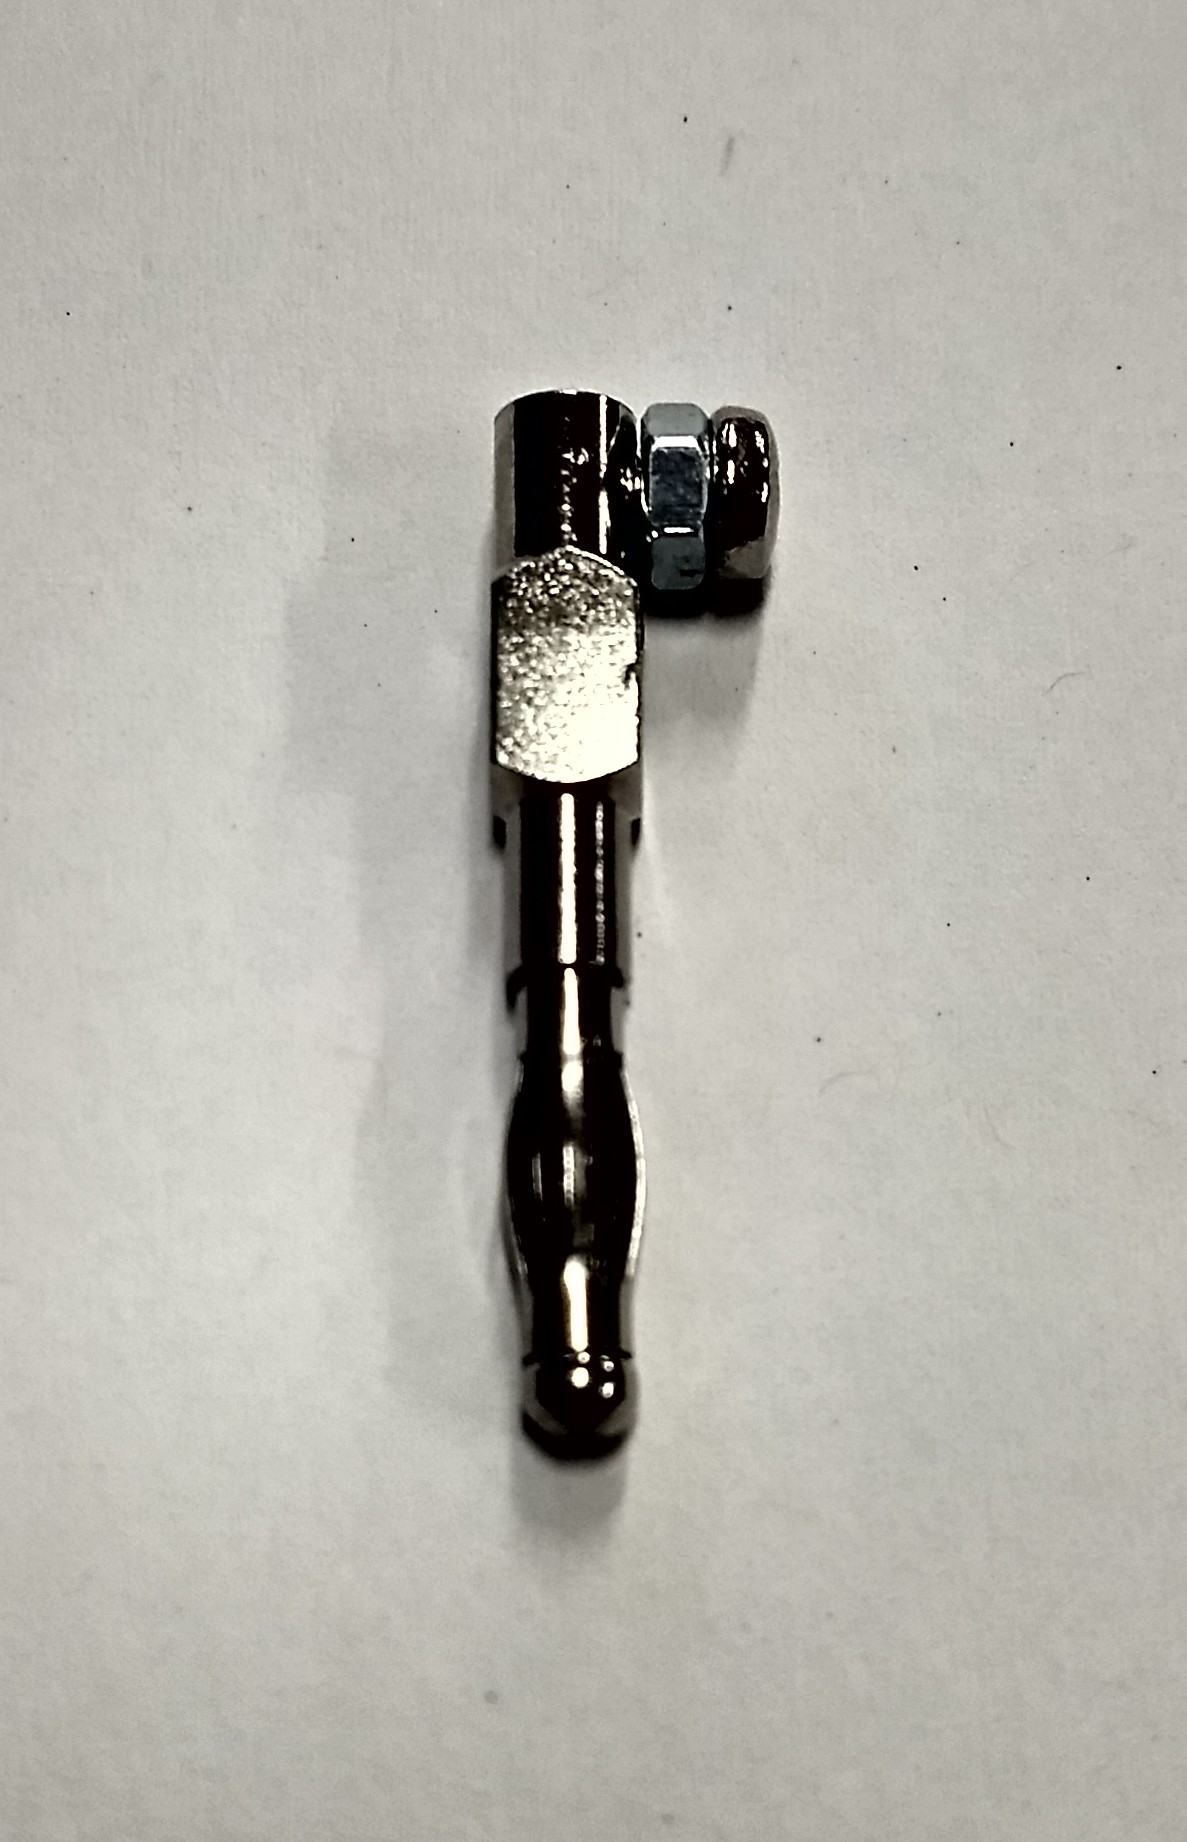
\includegraphics[width=0.3\linewidth]{banana.jpg}
    \caption{Banana plug mechanical fixing for MEMS sensors on vibration generator}
    \label{fig:Banana}
\end{figure}


\subsubsection{Results}

\begin{figure}
    \centering
    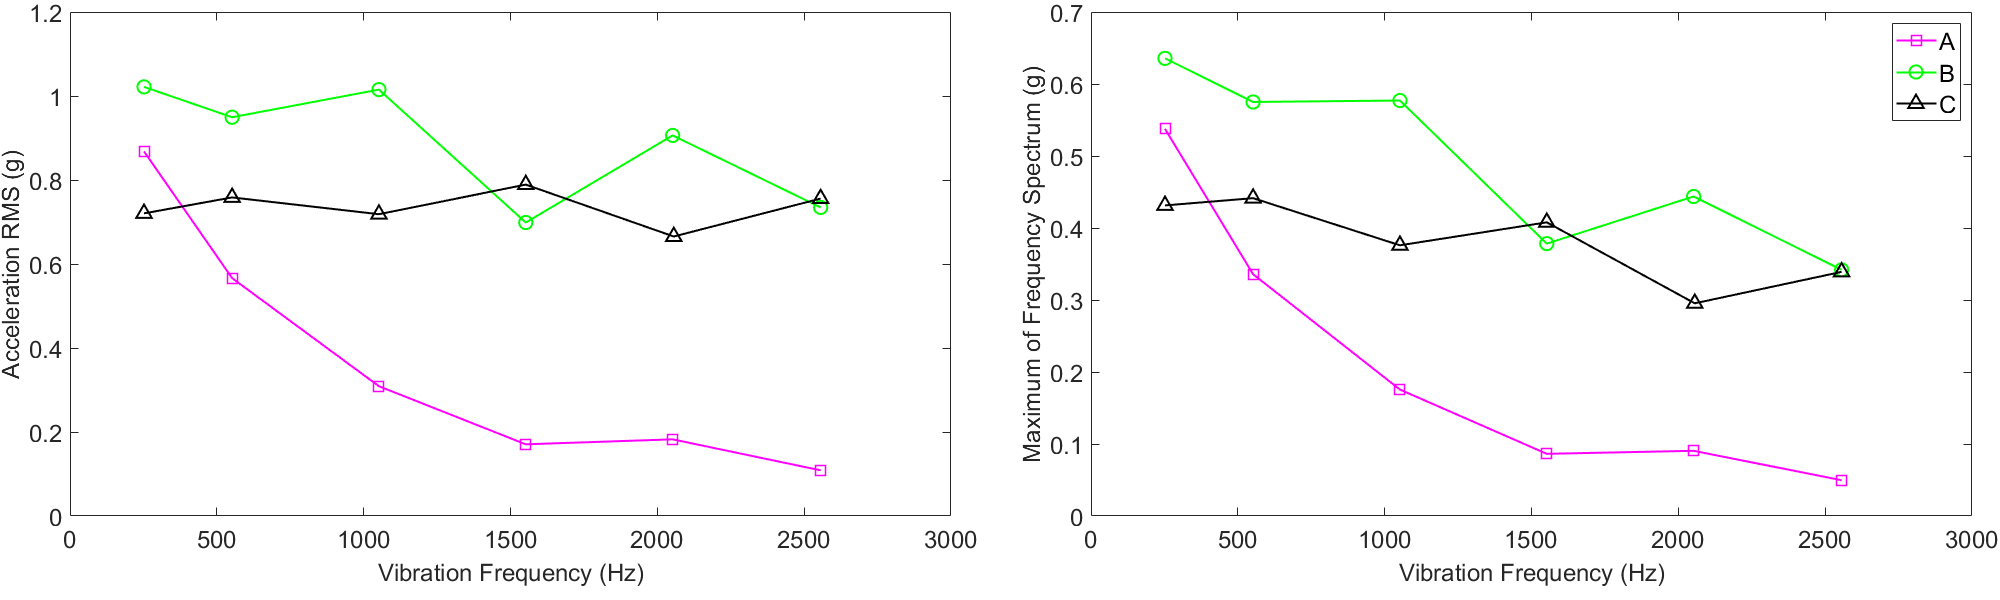
\includegraphics[width=\linewidth]{Acc_comparison.png}
    \caption{Comparison of RMS of acceleration and maximum of frequency spectrum for MEMS sensors across frequencies}
    \label{fig:Acc_comparison}
\end{figure}

\begin{figure}
    \centering
    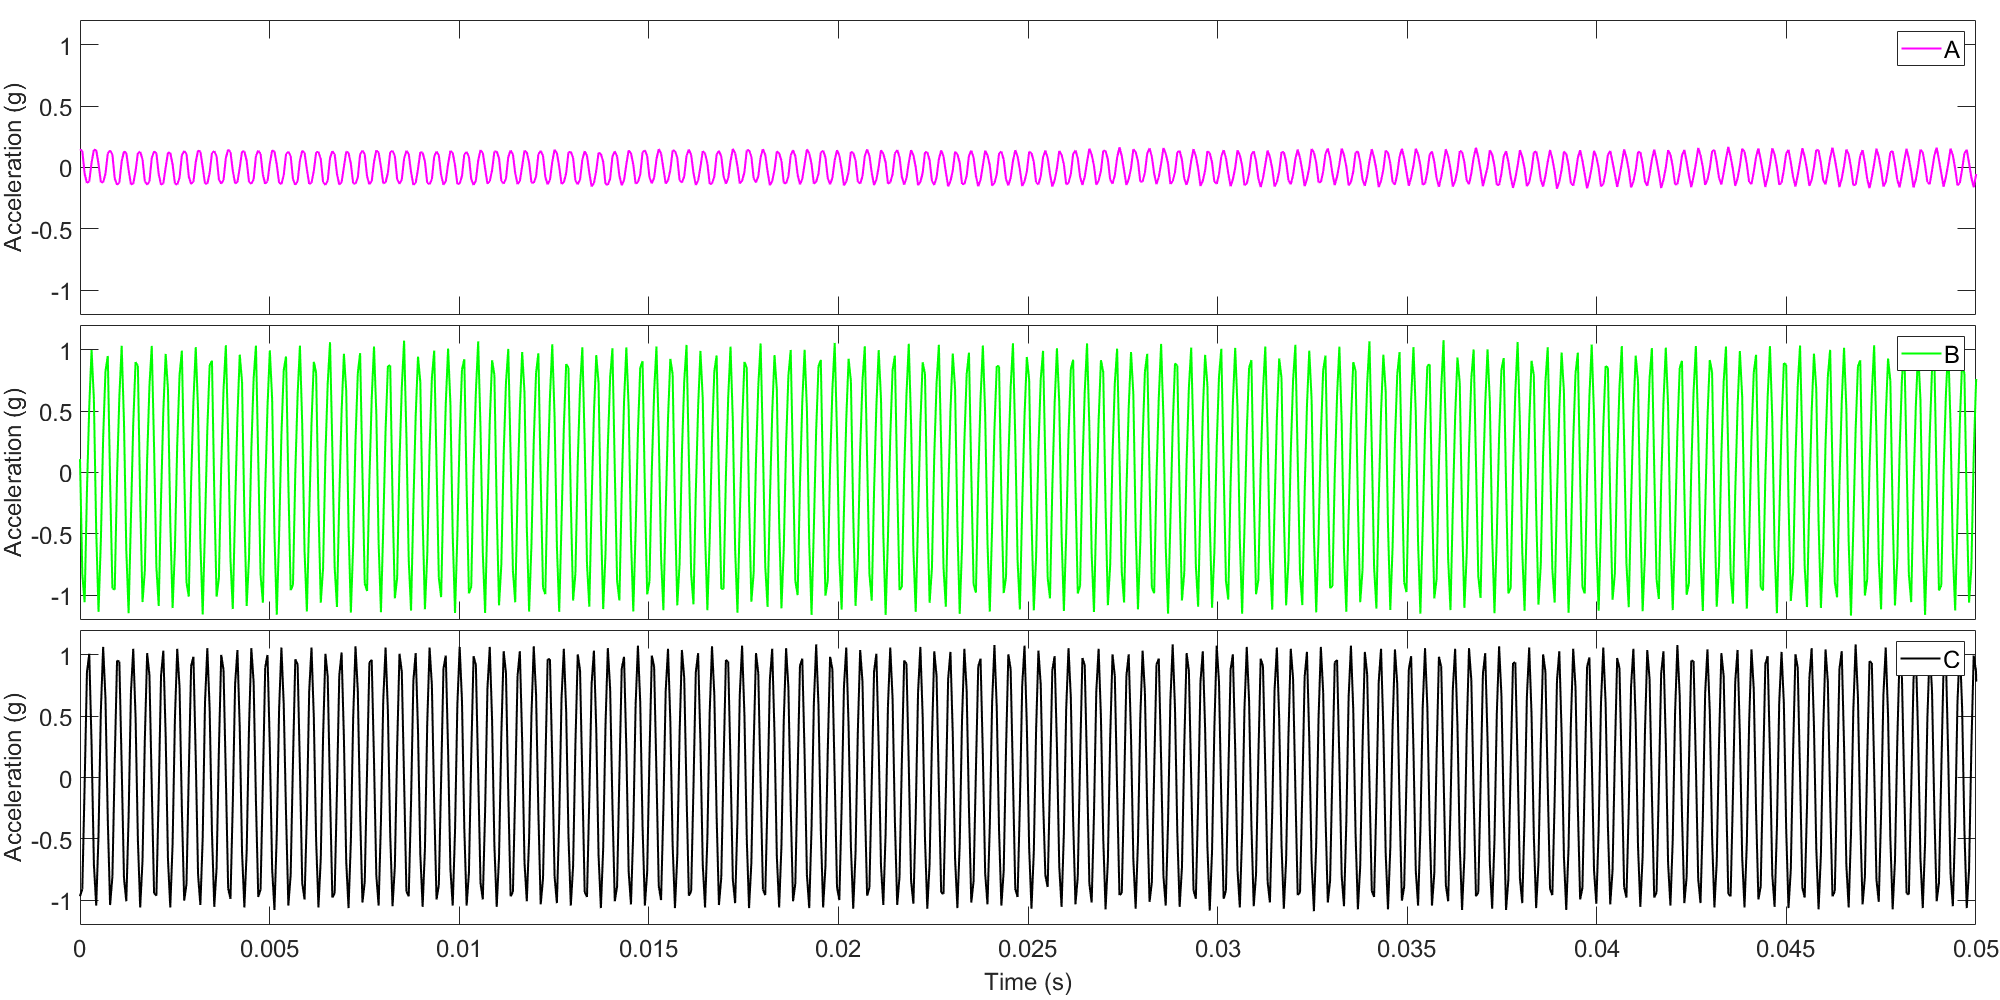
\includegraphics[width=\linewidth]{Acc_time_2553.png}
    \caption{Sample of time signal of MEMS sensors at 2553 Hz}
    \label{fig:Acc_time}
\end{figure}

\begin{figure}
    \centering
    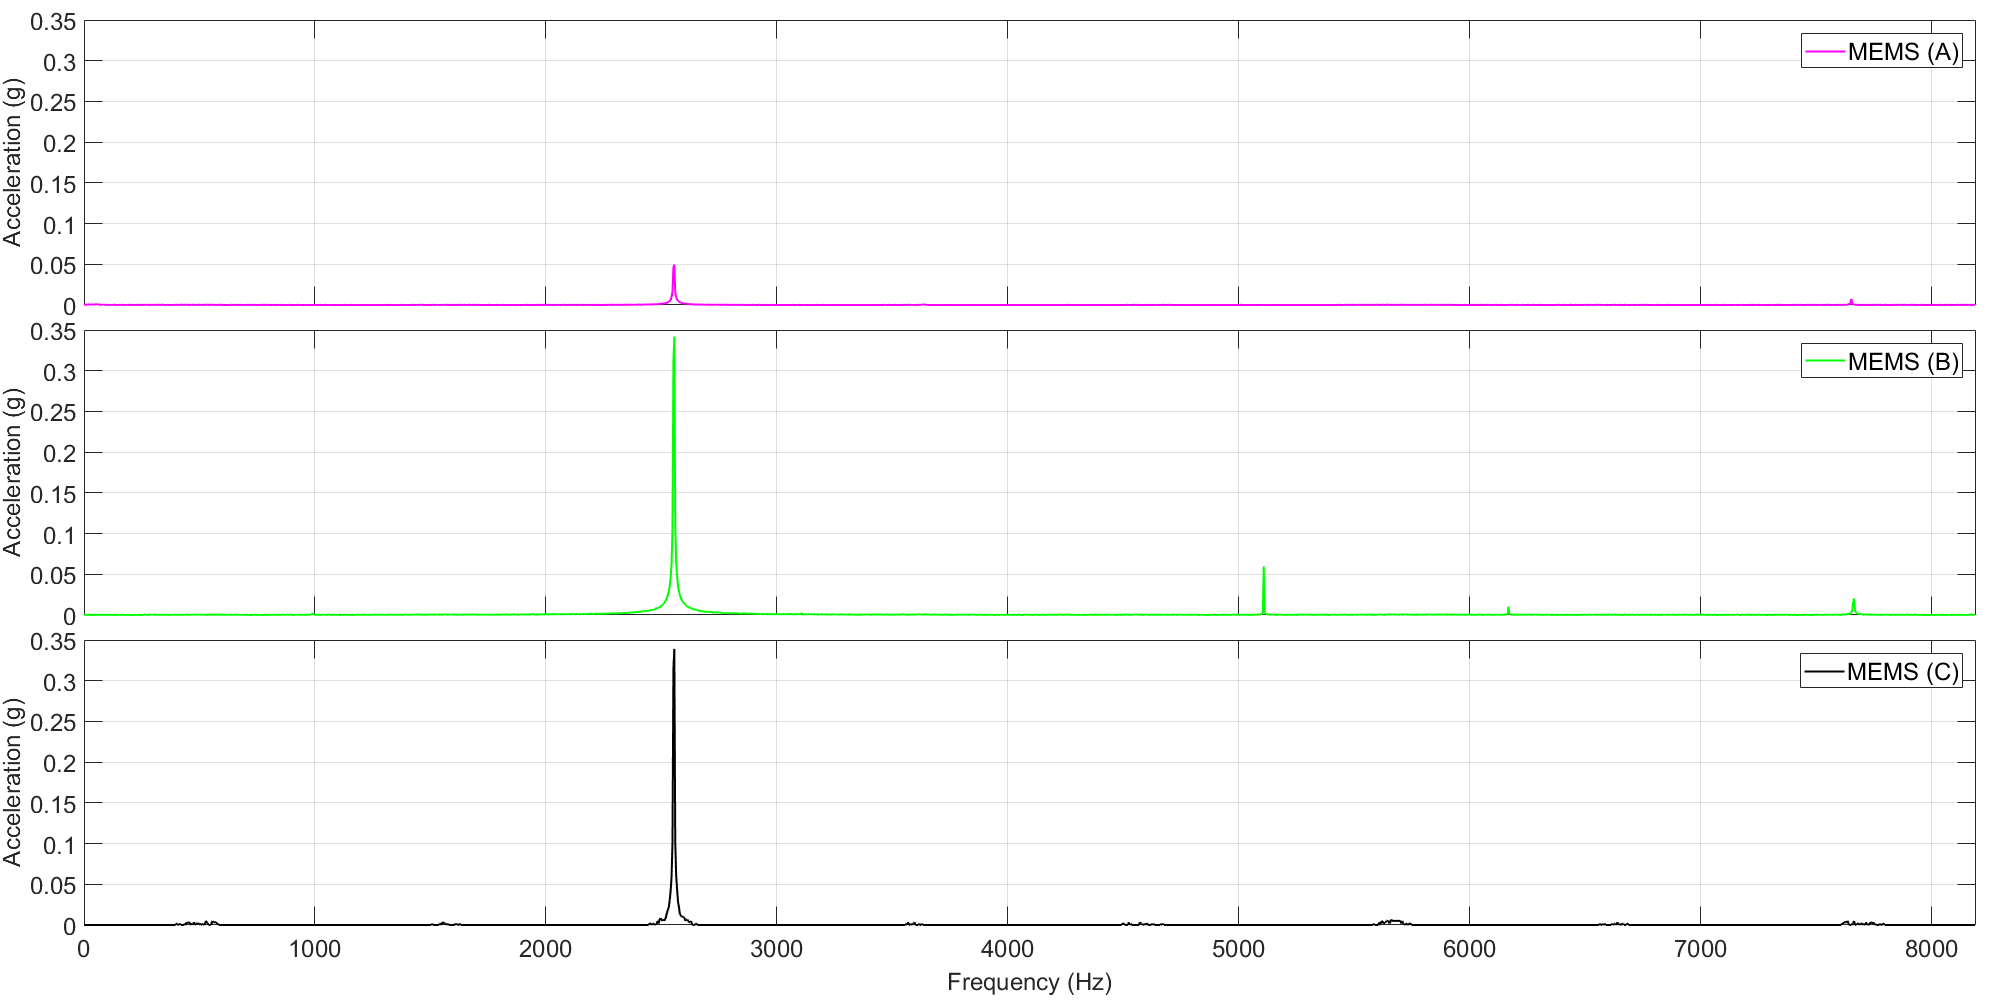
\includegraphics[width=\linewidth]{Acc_freq_2553.png}
    \caption{Averaged frequency spectrums for MEMS sensors at 2553 Hz}
    \label{fig:Acc_freq}
\end{figure}

The accuracy of the sensors cannot be directly derived from this test, as the exact acceleration produced by the vibration generator is not known.
However, MEMS C provided the most constant values for acceleration RMS and frequency spectrum maximum, followed by B (Fig \ref{fig:Acc_comparison}).
As expected, A performed similarly to the other sensors at the low frequency within its range but then quickly gave attenuated responses.
MEMS B and C had extremely similar responses at 2553 Hz, beyond the listed frequency range of B.
While it is promising that the calculated values were so close, the fact that this value is in the attenuated range of B suggests that it is not entirely accurate.
\par
Close inspection of the test at 2553 Hz (Fig \ref{fig:Acc_time}, Fig \ref{fig:Acc_freq}) highlight properties of the accelerometers which were also visible at other frequencies.
The time data for B and C is very similar and clean, and the attenuation for A is significant.
All sensors correctly identified the frequency with a sharp peak, and also showed some noise around 7.6 kHz, suggesting there may be some harmonics produced by the vibration generator.
B shows small peaks at several harmonics, possibly a result of the sensor harmonics or the board.
C shows harmonics and sub-harmonics, likely a result of noise given their small amplitude.
\par
This experiment should be repeated on a calibrated rig where the acceleration is known.
\par

The results suggest that C will be the most accurate and effective sensor for the embedded system, although it may struggle at low amplitudes.



\section{Current Sensors}


\begin{figure}
    \centering
    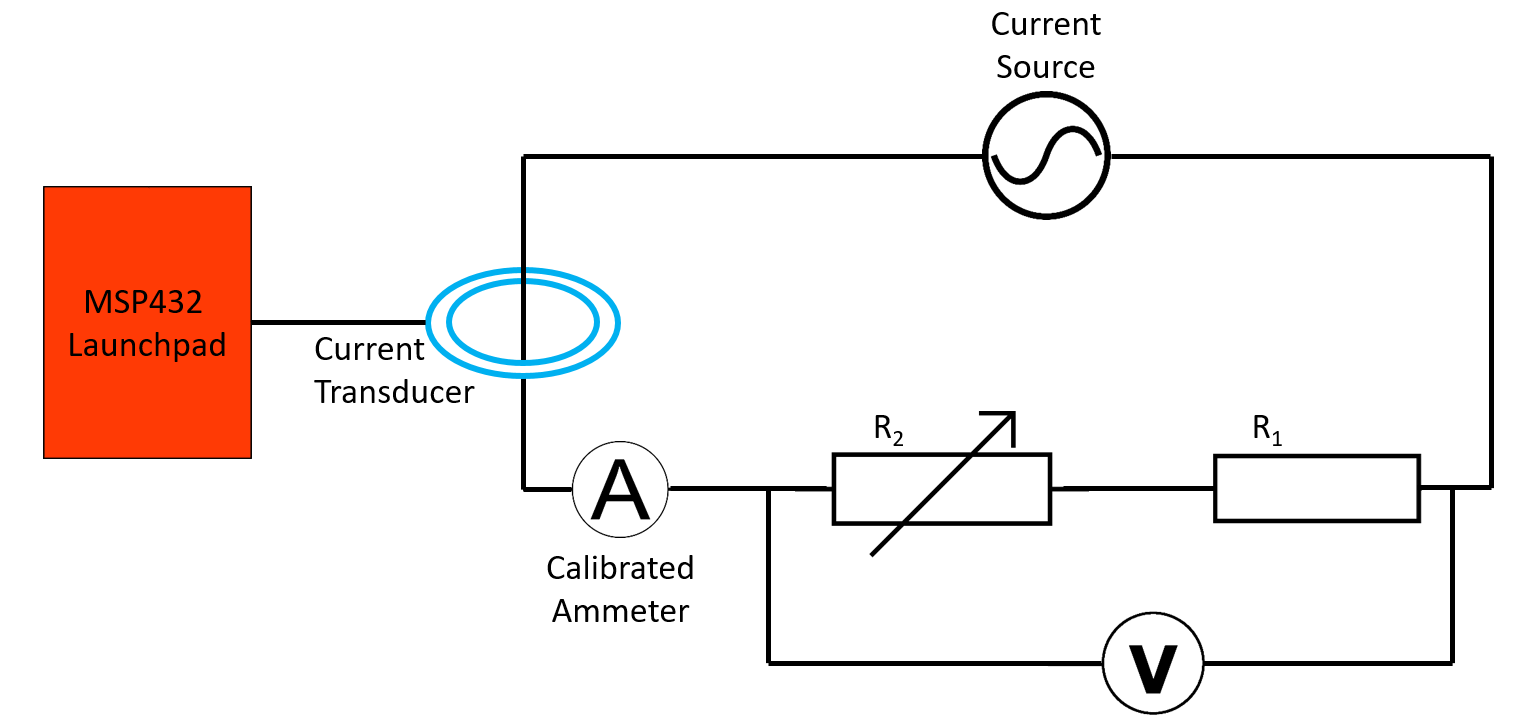
\includegraphics[width=\linewidth]{CurrentCalibrationTest.PNG}
    \caption{Test setup for validation of current transducers}
    \label{fig:CurrentCalibrationTest}
\end{figure}

\begin{savenotes}
\begin{table}
    \renewcommand{\arraystretch}{1.2}
	\begin{center}
	\begin{tabular}{lll}%Changed c to S
    	\toprule
        & \textbf{CT1} & \textbf{CT2}\\
        \midrule
        \textbf{Sensitivity (mV/A} & 76.67 & 13.333 \\
    	\textbf{Frequency Range (kHz)} & 250 & 100 \\
    	\textbf{Current Range (A)} & $\pm 20$ & $\pm 150$ \\
    	\textbf{Supply voltage (V)} & 3.3 & 5 \\
    	\textbf{Unit Price (£)\footnote{Unit price at large UK electrical retailer}} & 6.82 & 10.52 \\
        \bottomrule
    \end{tabular}
    \caption{Properties of current sensors tested for embedded system \cite{CT1}, \cite{CT2}}
    \label{tab:current_sensors}
    \end{center}
\end{table}
\end{savenotes}

Two Current Transducers (CTs) were selected as candidates for the embedded system (Table \ref{tab:current_sensors}).
A wider range of available sensors were found to be available than for accelerometers.
The sensitivity of the sensors varies largely, allowing for the embedded system to monitor the current of differently sized motors on board ships.
Both CTs selected are open loop, hall-effect probes which can be easily applied to a variety of motors, needing only to isolate a single phase.
The frequency range of both CTs is above what will be required for the embedded system, providing the capability in hardware for future advancements of the system focusing on higher frequencies.
Notable differences between the CTs is the current range and supply voltage.
Having a large current range allows for application to a wider range of machinery, including larger pumps found on board ships, at the possible cost of decreased accuracy for lower power machines.
A supply voltage of 5 V, required by CT2, can be accomodated by the embedded system but to allow full use of the current range circuit protections and scaling of the signal would be required as the embedded system will use 3.3 V analogue reference voltage and signals beyond that range could cause damage.
\par
The sensors were tested by generating an AC current and passing it through resistors to generate a known current level (Fig \ref{fig:CurrentCalibrationTest}).
Step down transformers were used to provide large currents at mains frequency (50 Hz in UK) and around 30 V peak.
Large ceramic resistors with sizeable heat sinks were connected in series with a variable resistor and an ammeter to adjust the current to the required values.
A moving iron AC ammeter certified to half a percent provided confidence in the current \cite{Ammeter_certificate}.
The current transducer was then placed around the wire connecting the ammeter to the current source.
A voltmeter was connected across the load for safety and to note any anomalies.
\par
The current was set to 1 A, 2 A and 3 A and three measurements were taken for both sensors of 4096 points at 4096 Hz.
A lower sampling rate was chosen than for the accelerometers to provide increased resolution around the supply frequency.
The data was transformed to the frequency domain on-board.
Time and frequency data was transferred to a computer for further processing and storage.
The average RMS of time signal was calculated across the three samples and converted to SI units using the theoretical sensitivity of the sensors.
The measured sensitivity was then calculated using the known current values for comparison to the theoretical values.
The frequency spectrums were also averaged to remove impulses and other local effects.
\par
A large peak is expected at 50 Hz with some small peaks at harmonics.
Other experiments were taking place in the High Voltage Zepler Laboratory so could provide a source of noise in the data.
There will be some variation in results due to changes in temperature.




\subsubsection{Results}

The CTs tested performed very differently.
CT1 provided very clean results (Fig \ref{fig:CurrentCalibration}) with no harmonics or noise visible in the time data or frequency spectrum.
CT2 did not perform as well showing a lot of noise in the time data and a small amount of noise in the frequency spectrum, .
The frequency spectrum shown for both CTs has been abbreviated to the area of interest, no useful signals were seen above 200 Hz.
Both sensors clearly highlight the expected peak at 50 Hz with no sign of significant harmonics.
\par

The calculated and measured sensitivities of the sensors are listed in Table \ref{tab:current_calibration}.
CT1 performed very closely to its theoretical sensitivity, whereas CT2 had a much lower measured sensitivity than its theoretical value.
This could be due to the relatively low current compared to the range of CT2, or could be a result of sensor inaccuracy.
\par
This experiment should be repeated at higher currents and with varying supply frequency to evaluate how the CTs perform across a range of frequencies more suited to CBM.
\par

The results suggest that CT1 is the more appropriate CT for the embedded system, assuming that the current requirements are within its current range.
Beyond that current range, CT2 can still be expected to accurately describe the shape of the frequency spectrum, although its scale may not be relied on as heavily.

\begin{table}\centering
    \begin{tabularx}{\textwidth}{@{}*{1}{>{\centering\arraybackslash}X}l*{2}{>{\centering\arraybackslash}X}l*{2}{>{\centering\arraybackslash}X}@{}}\toprule
    \textbf{Current (A)} &  \phantom{a} & \multicolumn{2}{c}{\textbf{CT1}} & \phantom{a} & \multicolumn{2}{c}{\textbf{CT2}}\\
    \cmidrule{3-4} \cmidrule{6-7}
    && RMS (A) & Sensitivity (mV/A) && RMS (A) & Sensitivity (mV/A)\\
    \midrule
    1.0 && 1.001 & 77.3 && 0.665 & 8.9 \\
    2.0 && 2.014 & 77.2 && 1.273 & 8.5 \\
    3.0 && 3.024 & 77.3 && 1.820 & 8.1 \\
    \bottomrule
    \end{tabularx}
\caption{Results of current sensor testing}
\label{tab:current_calibration}
\end{table}

\begin{figure}
  \centering
  \begin{subfigure}[b]{\linewidth}
    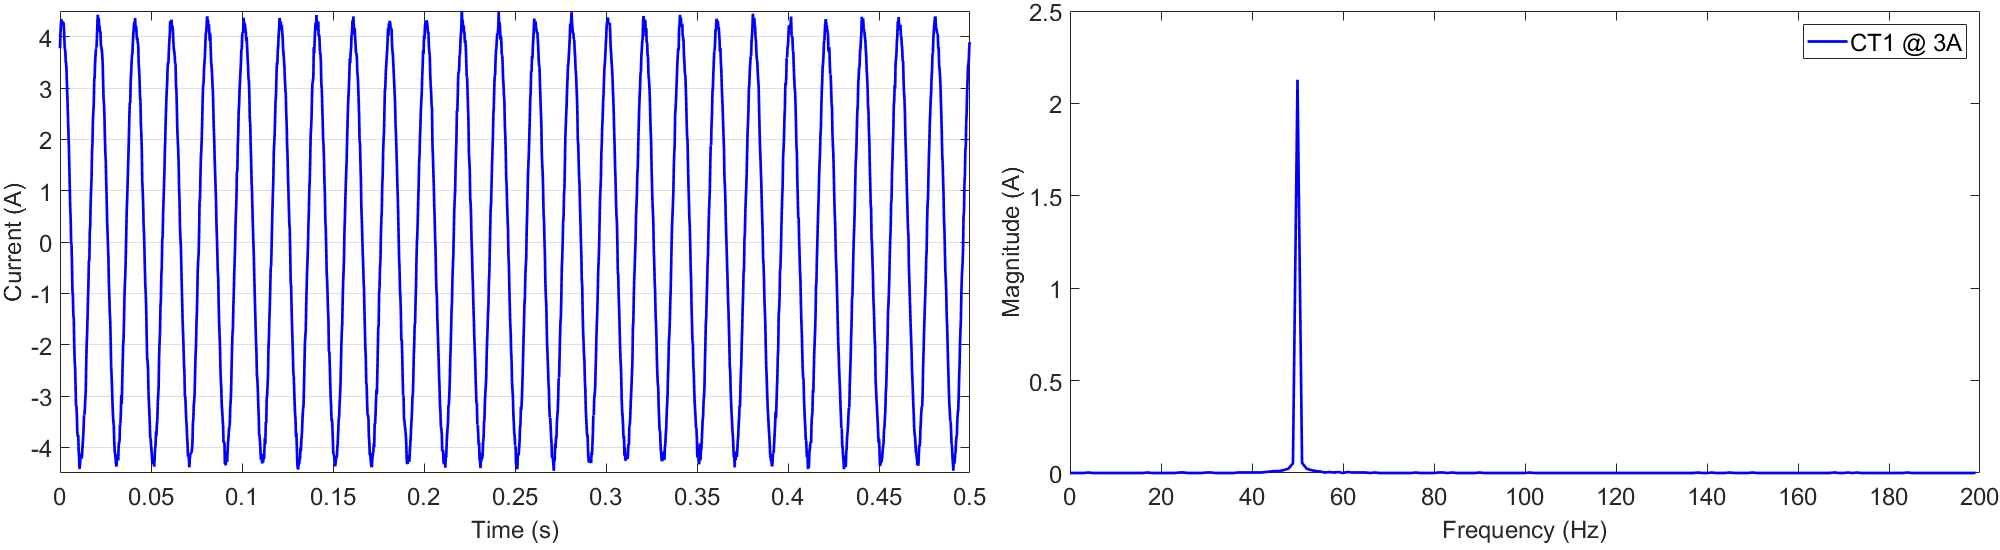
\includegraphics[width=\linewidth]{Current_3A_small.png}
    \caption{Results of 3 A current test for CT1}
  \end{subfigure}
  \begin{subfigure}[b]{\linewidth}
    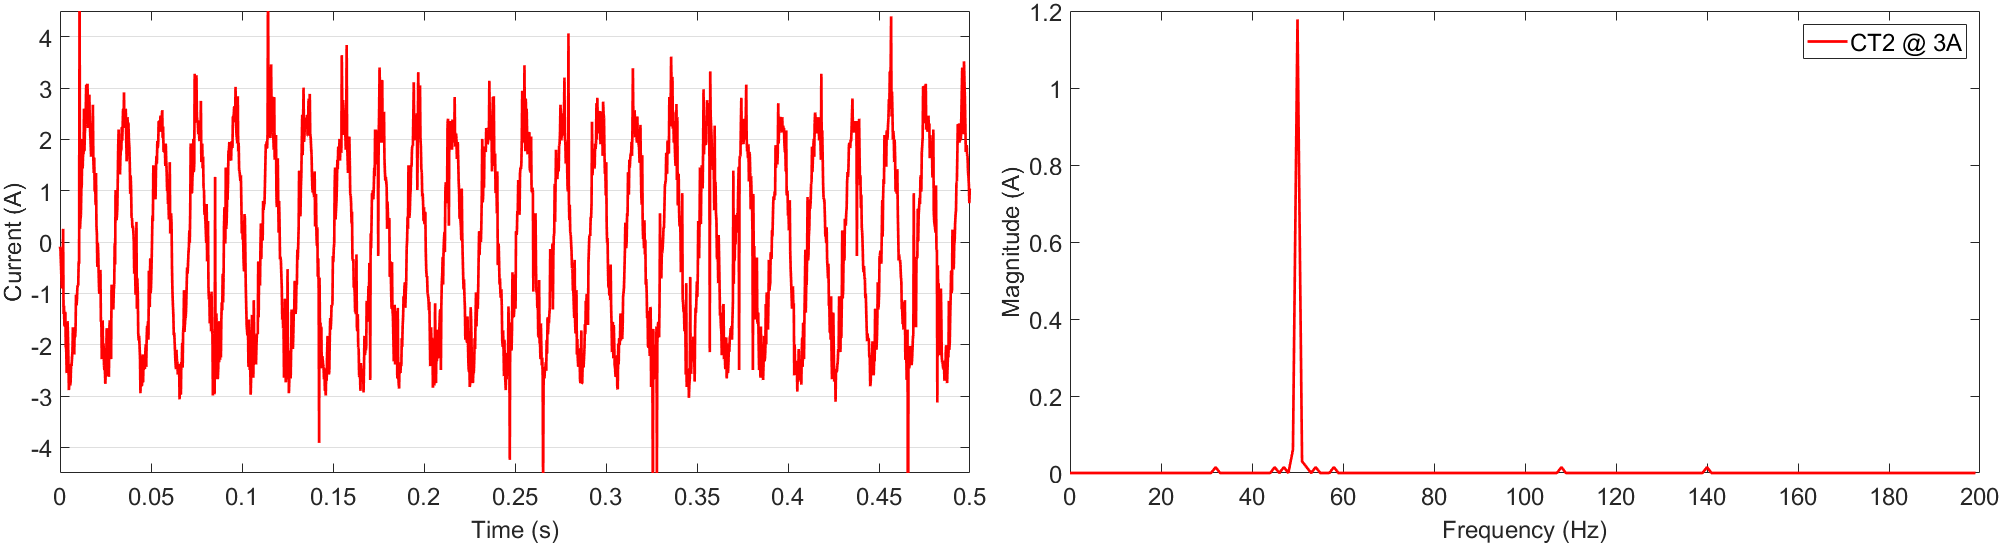
\includegraphics[width=\linewidth]{Current_3A_big.png}
    \caption{Results of 3 A current test for CT2}
  \end{subfigure}
  \caption{Current Test at 3A}
  \label{fig:CurrentCalibration}
\end{figure}
